\subsection*{a)}
	Using the law of mass action, we can say that the product of our majority and minority carrier concentrations (holes and electrons, respectively) is equal to the square of the intrinsic carrier concentration, $n_i$. Since $n_i^2 = N_C N_V \exp\left(\dfrac{-E_g}{k_B T}\right)$, $n_i$ has a value of $6.57 \times 10^{9} \textrm{ cm}^{-3}$ in silicon, at room temperature. This holds so long as the base region is large, and hence the emitter and collector can be ignored. Under an assignment amendment, the value of $n_i = 1.0 \times 10^{10}$ will be used.
	
	We can take the majority carrier concentration, $p_{p0}$, to be approximately $N_A = 10^9 \textrm{ cm}^{-3}$, and so our minority carrier concentration must be $n_{p0} = \dfrac{n_i^2}{p_{p0}} = \dfrac{10^{20}}{10^{19}} = 10 \textrm{ cm}^{-3}$.
\subsection*{b)}
	The minority carrier concentration can be expressed as
	$$\Delta n(x) = 
	\Delta n_2 \frac{\sinh\left(\frac{W_B - x_b}{L_n}\right)}{\sinh\left(\frac{W_B}{L_n}\right)} + 
	\Delta n_3 \frac{\sinh\left(\frac{x_b}{L_n}\right)}{\sinh\left(\frac{W_B}{L_n}\right)}
	$$	
	where
	\[
		\begin{aligned}
		\Delta n(x_b) &= n(x_b) - n_{p0} \\
		\Delta n_2  &= n(0) - n_{p0} \\
		\Delta n_3  &= n(W_B) - n_{p0} \\	
		\end{aligned}
	\]
	
	If we treat the base-emitter and base-collector regions as two separate diodes, we can define the minority carrier concentration at the interfaces of the transition regions from the base side as follows: \\
	
	\noindent For the base-emitter junction
	$$\Delta(x_b = 0) = \Delta n_2 
			= \frac{n_i^2}{N_A}
			 \left(
				\exp{\left(
					\frac{- q V_{BE}}{k_B T}				
				\right)} - 1
			\right)
	$$
	For the base-collector junction
	$$\Delta(x_b = 0) = \Delta n_3
	= \frac{n_i^2}{N_A}
	\left(
		\exp{\left(
			\dfrac{q V_{BC}}{k_B T}				
		\right)} - 1
	\right)
	$$
	
\subsection*{c)}
	\begin{figure}[htbp!]
		\centering
		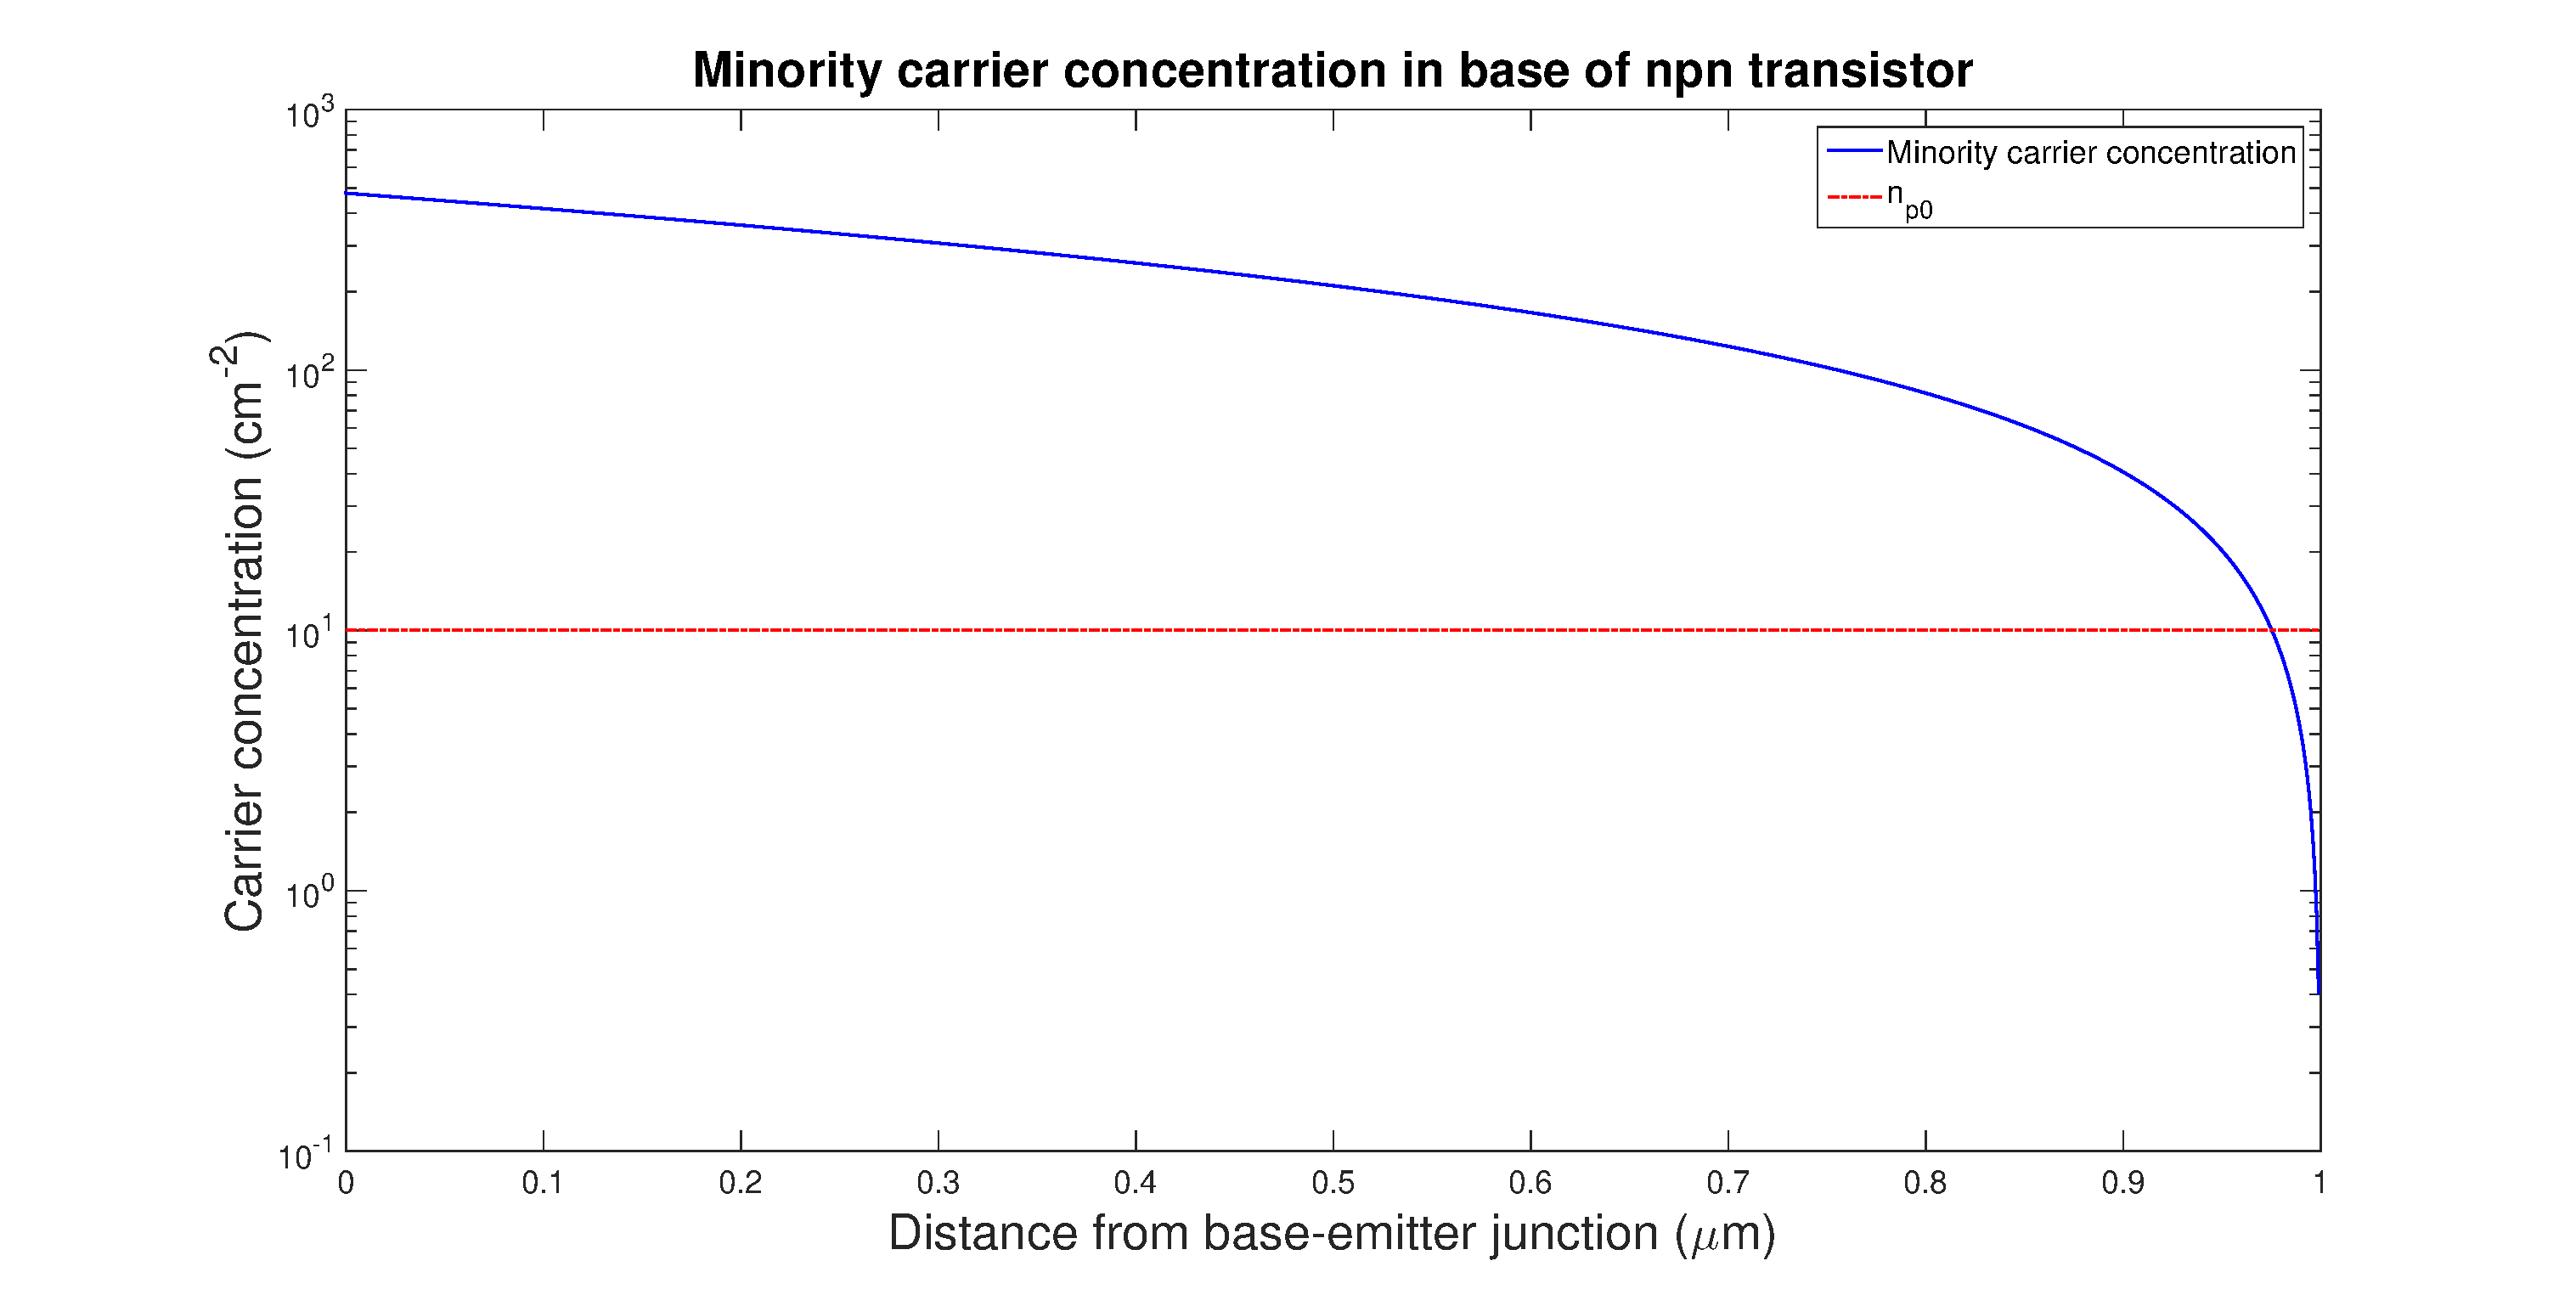
\includegraphics[width=0.8\textwidth]{./img/3c}
		\caption{Minority carrier concentration for a base width $W_B = 1 \mu m$.}
	\end{figure}
\subsection*{d)}
	\begin{figure}[htbp!]
		\centering
		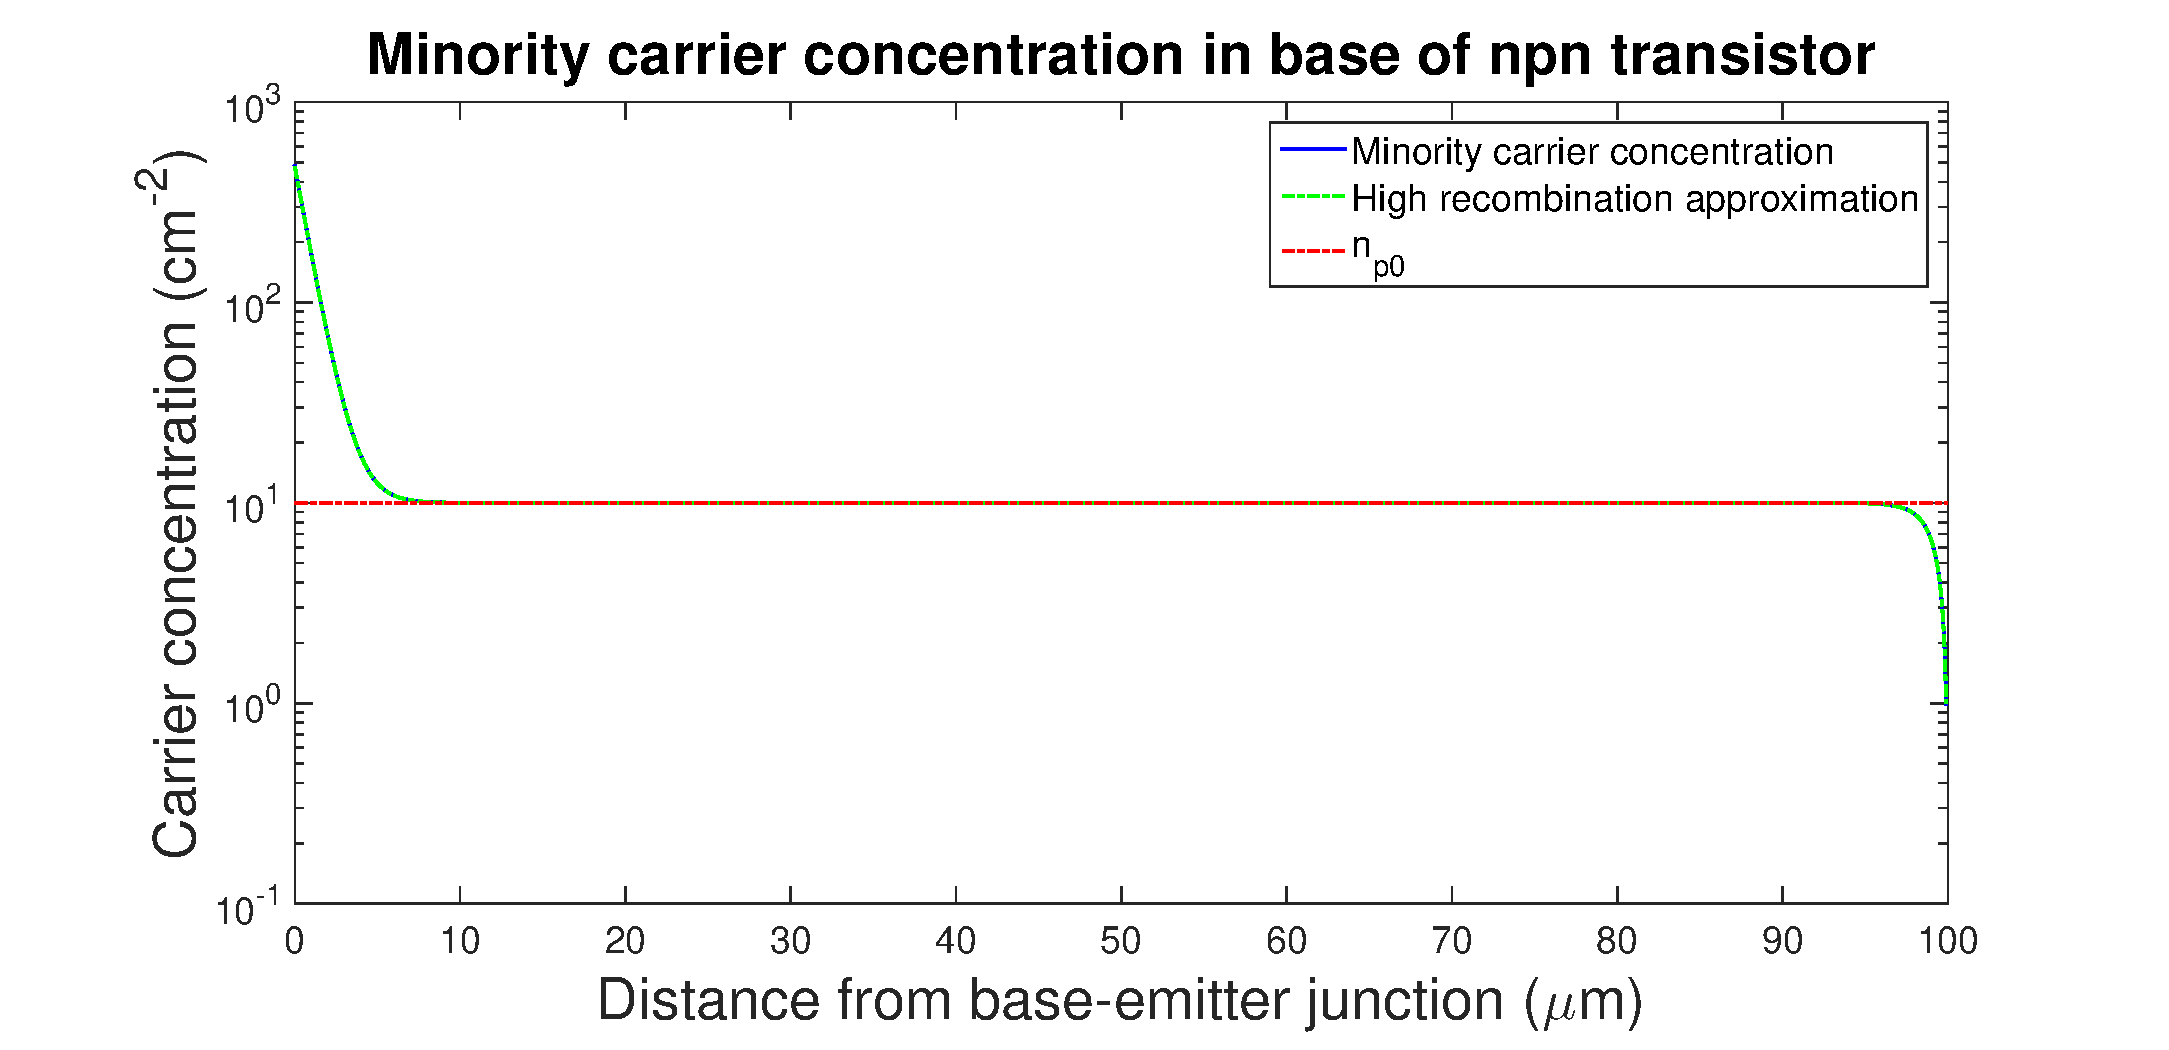
\includegraphics[width=0.8\textwidth]{./img/3d}
		\caption{Minority carrier concentration for a base width $W_B = 100 \mu m$.}
	\end{figure}
\subsection*{e)}
	\begin{figure}[htbp!]
		\centering
		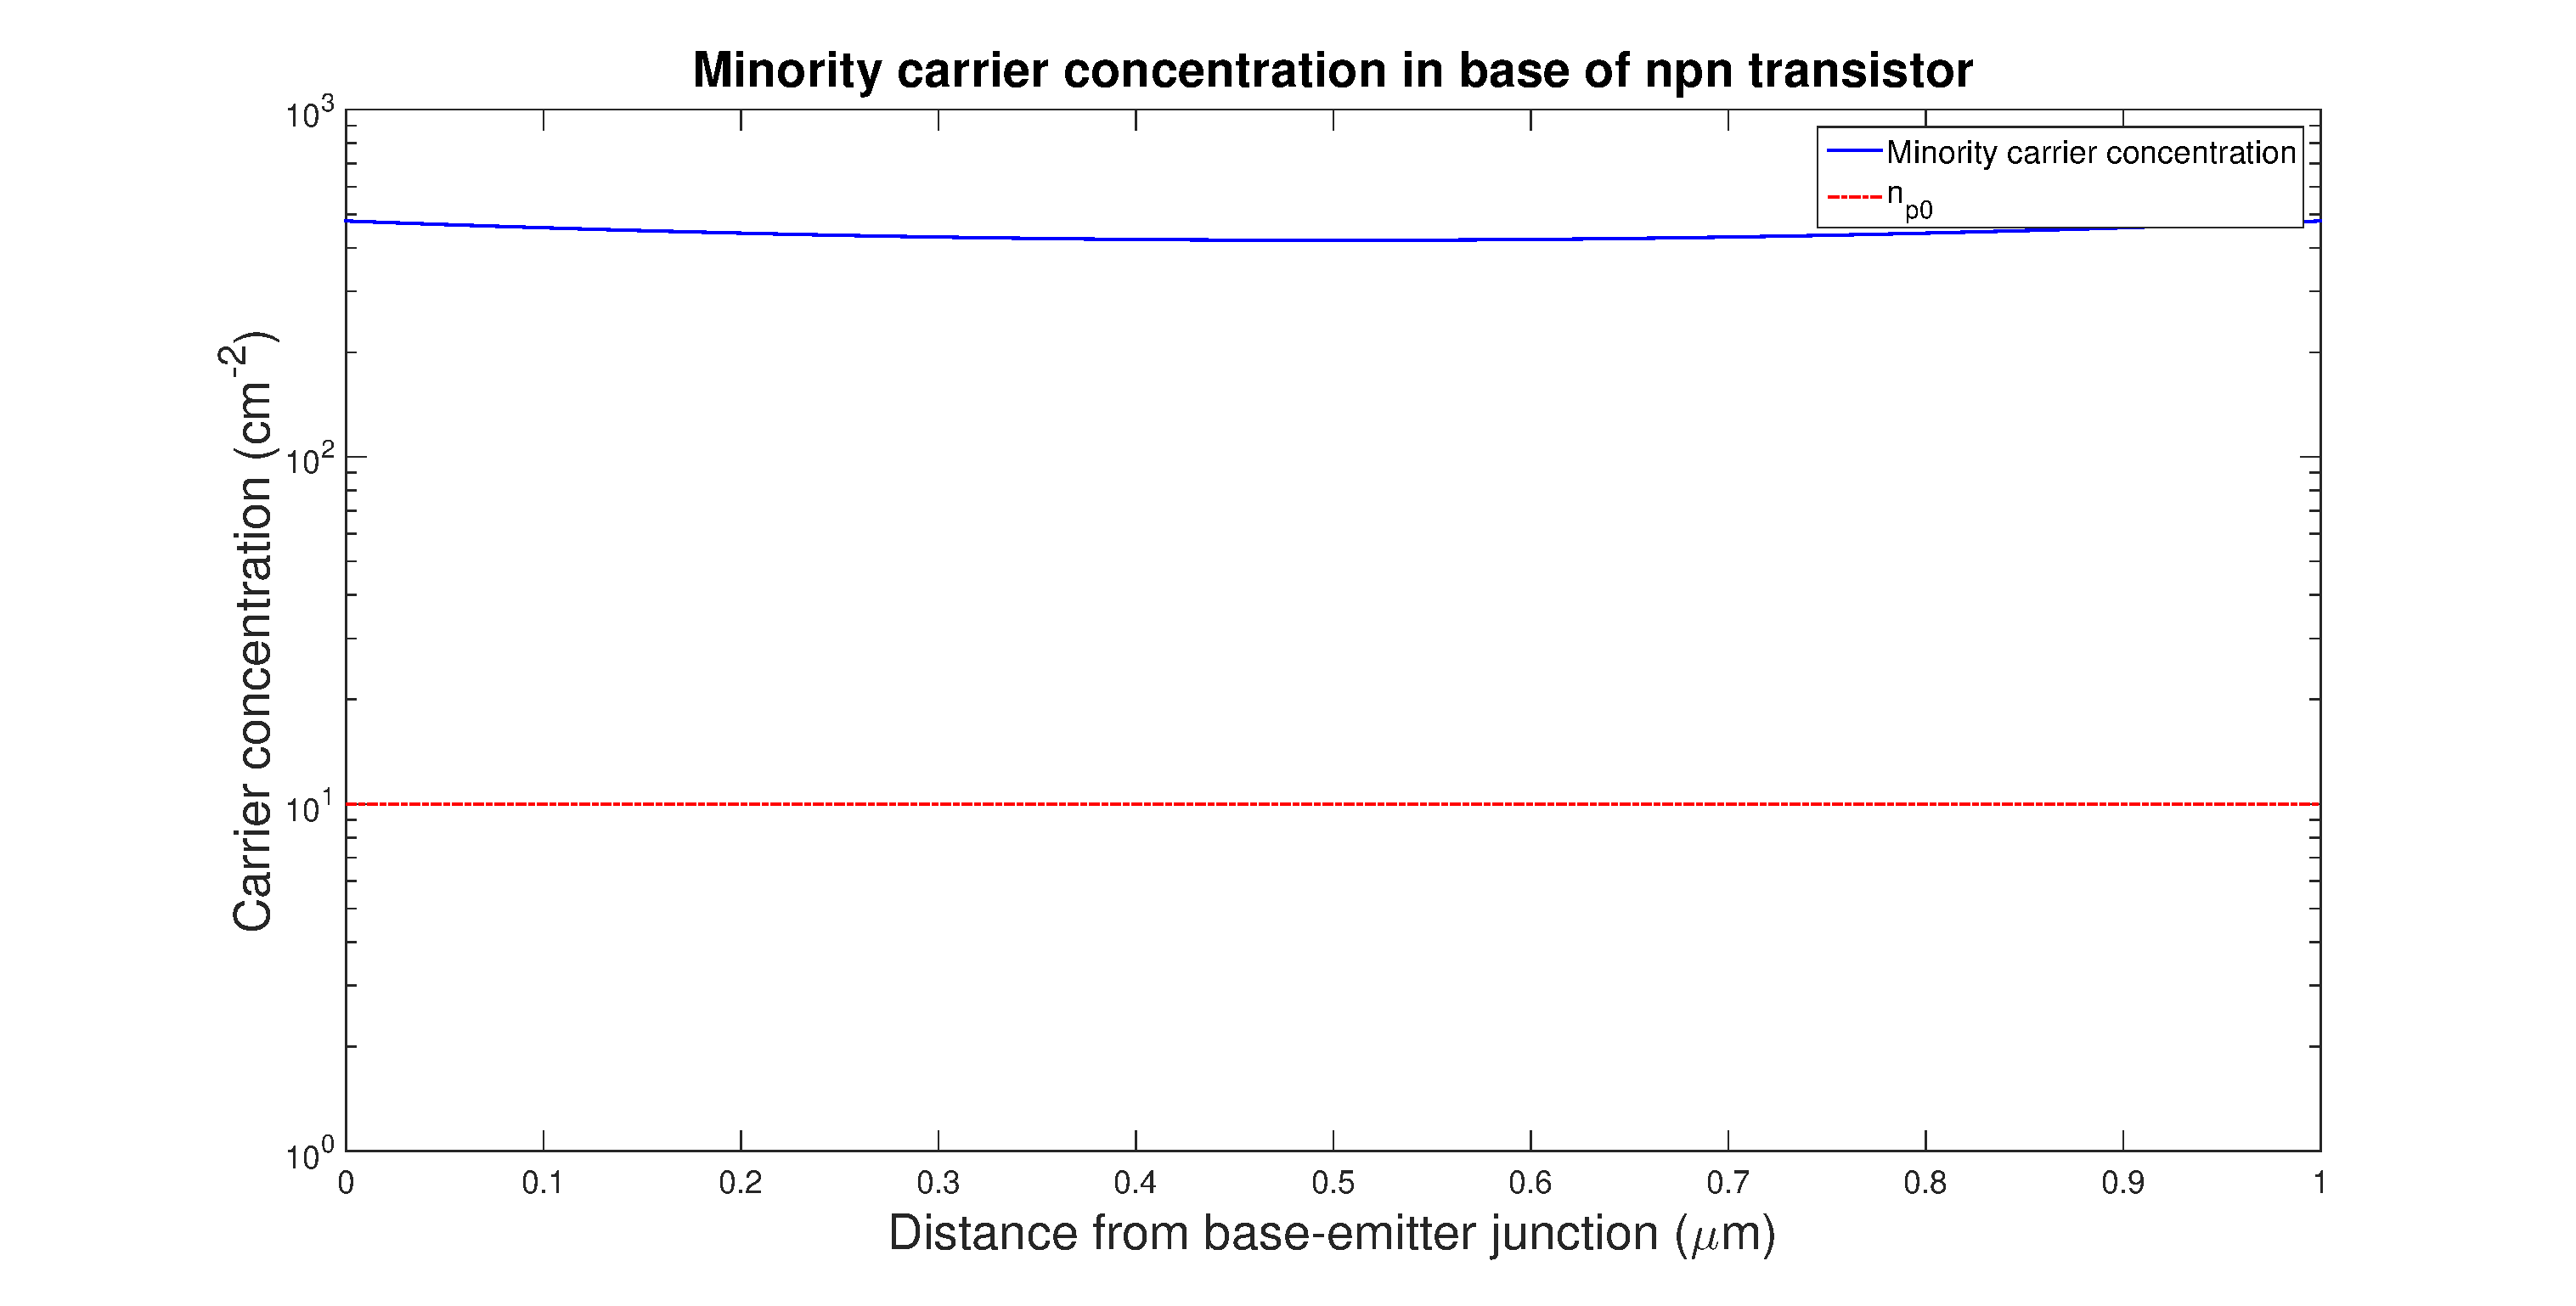
\includegraphics[width=0.8\textwidth]{./img/3e}
		\caption{Minority carrier concentration for a base width $W_B = 1 \mu m$, operating in saturation with $V_{BC} = 0.1 \textrm{ V}$.}
	\end{figure}